\chapter{基于语料资源的中文情感词典扩展}
\label{ch3}

\section{引言}

自然语言中,一个词语的语义极性(semantic polarity)表示它对于其语义组(semantic group)或词汇场(lexical field)范式的偏离方向\upcite{Hatzivassiloglou1997}。在自然语言处理领域,情感分析(Sentiment Analysis)能够使用计算手段自动从自然语言中发现观点和情感等主观信息\upcite{Liu2012,Pang2008OMS},通常会使用一些标注了极性(积极或消极)的词汇构成的情感词典资源。研究如何能够通过计算方式获得词语的语义极性,自动构建情感词典一直得到计算语言学和自然语言处理研究人员关注。在英文情感词典构建中,Wilson等\upcite{Wilson2005,Wilson2009}对一些单词进行了人工极性类别的标注形成了OpinionFinder词典;Bradley等\upcite{Bradley1999}标注了并发布了情感范式的英文词典ANEW,后来Nielsen等\upcite{Nielsen2011}在Twitter语言上应用并自动扩展了ANEW,形成AFINN词典。Esuli和Sebastiani\upcite{Esuli2006}以及后来Baccianella等\upcite{Baccianella2010}在著名的语义词典Wordnet基础上采用自动计算的方式开发出了情感词典SentiWordnet。Thelwall等\upcite{Thelwall2012}设计实现了能对词语的情感强度进行估计的方法。情感也可以通过创建情绪词典来进行计算,Plutchik情绪轮提出了四对对立的情绪状态:joy-trust,sadness-anger,surprise-fear和anticipation-disgust\upcite{Plutchik2001}。Mohammad和Turney\upcite{Mohammad2013b}根据Plutchik情绪轮分类方法使用情绪分值标注了一些词语形成NRC情绪词典。在2013和2014年举办的SemEval(Semantic Evaluation)评测中,NRC-Canada队利用NRC词典并扩展出两种新的词典,取得了最好成绩\upcite{Mohammad2013,Kiritchenko2014}。为了克服以上语法层面建立的词典的上下文语境以及领域适应性问题,一些学者提出了基于概念(concept-based)构建情感词典\upcite{Tsai2013},其中SenticNet是使用常识知识库建立的公开可用的基于概念的情感词典\upcite{Cambria2014}。

中文情感分析研究起步较晚,想对于丰富的英文情感词典资源,缺乏普遍认可的可靠的中文情感词典。目前研究使用主要有HowNet情感词典\upcite{2013},NTUSD情感词典\upcite{Ku2007}以及大连理工大学的情感词汇本体词库\upcite{2013a}。这些词典主要是以手工或半自动方式编辑而成。我们的前期工作提出了根据语义词典HowNet语义关系将英文情感词典跨语言转换为中文情感词典的方法,并构建了带有极性标示以及极性强度值的的情感词典SentiHowNet\upcite{谢松县2014}。
基于语义词典的情感词典构建方法是一种常用的情感词典构建方法。采用这种方法的优势在于可以比较容易获取情感词语,基于词语的语义关系也易于进行情感极性计算。但是,基于语义词典的情感词典构建方法受限于语义词典的规模和语义关系的定义,而且对于专业领域中不断涌现的新词语,对情感词典的覆盖度提出了严峻的挑战。随着互联网应用,尤其是社交媒体的不断涌现,越来越多的用户在各种网络平台上发布信息,网络上的用户产生内容(User Generated Content,UGC)不断涌现,研究如何利用这些丰富的网络语料对情感词典进行自动扩展具有十分重要的意义。

本章提出的基于语料资源的无监督的情感词典扩展方法,可以使用于无需标注的网络数据语料对中文情感词典进行自动扩充。

\section{问题描述}
基于语料资源的情感词语选择与极性计算,在英文中相关研究通常有两种实现思路:一是基于语言特征的方法,例如,Hatzivassiloglou\upcite{Hatzivassiloglou1997}等人采用并列或转折连词来判断新的情感词并计算其极性。二是基于统计特征的方法,例如,Turney等\upcite{Turney2002}采用点互信息统计学方法从语料中发现共现度高的情感词并计算其极性。基于以上情感词语选择与极性计算方法的分析,本文将基于中文语料资源扩展情感词典时需要解决的问题描述如下:

\begin{enumerate}
\item 研究根据中文语言中的并列、递进以及转折关系对情感词的发现以及极性计算的作用;
\item 根据中文特点,基于统计特征相关知识设计情感词语选择和极性计算方法;
\item 研究采用基于语言特征和统计特征相混合的方式进行情感词语选择和极性计算。
\end{enumerate}

\section{数据集及预处理}
本文使用的数据资源如表~\ref{tab3-1}所示,选取的语料资源是谭松波博士提供的酒店、书籍和电子商品评论三个领域的语料文本各4000篇\upcite{Lin2012}。
\begin{table}[htp]
\centering
\caption{数据集及词典资源}
\label{tab3-1}
\begin{tabular}{|l|l|l|}
\hline
词典 & SentiHowNet &基于前期工作\upcite{谢松县2014}\\
\hline
\multirow{3}{2cm}{语料} & Hotel & 4000篇\\
                     & Book & 4000篇\\
                     & NoteBook & 4000篇\\
\hline
\end{tabular}
\end{table}

其中对语料进行预处理需要将中文文本进行分词并进行词性标注。中文分词处理是对语料进行进一步处理的基础,采用的是中科院设计实现的ICTCLAS分词软件\upcite{张华平2014};然后将词性标注为形容词(ADJ)和副词(ADV)的,在SentiHowNet\upcite{谢松县2014}中出现的进行极性和极性值标注;生成的结构化语料预处理记录格式如图~\ref{fig3-1}所示,主要有词语编号(ID)、词性(Category)、中文词语(W\_C)、词语在句子中的编号(Word\_Tag)、词语所在语料文件编号(File\_Tag)、词语所在句子编号(Sentence\_Tag)、极性标注(Senti\_Tag)、积极极性值(PosScore)和消极极性值(NegScore)。值得说明的是,极性标注的取值为Yes和No,分别表示已标注和未标注,可以用于在具体的计算过程中直接进行情感词语的选择。

\begin{figure}[htp]
\centering
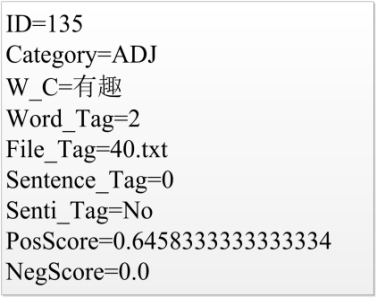
\includegraphics[height=95pt]{3-1.png}
\caption{语料预处理记录格式}
\label{fig3-1}
\end{figure}

\section{基于语言特征的情感词典扩展}
早期对于英文语言特征一些研究\upcite{Hatzivassiloglou1997}发现,由连词(如and或but)连接的两个形容词的极性往往存在一定的关联性,如“and”连接的形容词(如“nice and good”)极性相同,而“but”连接的形容词(如“nice but unnatural”)极性相反。而对于中文来说,基于语言特征的中文情感词是否会遵循想通的规律,非常值得进行研究。

\subsection{连词选择}
连词是用来连接词与词、词组与词组或句子与句子、表示某种逻辑关系的虚词。连词可以表示并列、承接、转折、因果等关系。本文主要研究基于表达并列、转折和递进三种关系的连词如何影响情感词的极性计算,选择的连词为:
\begin{itemize}
\item \textbf{并列关系连词:}和、跟、与、既、同、及、况、况且、乃至、并、也、又;
\item \textbf{转折关系连词:}却、虽然、但是、然而、偏偏、只是、不过、至于、致、不料、岂知;
\item \textbf{递进关系连词:}不但、不仅、何况、并、且、而且。
\end{itemize}

\subsection{基于连词的极性计算}
基于连词的情感词语极性计算基本思路是,待标注词语的极性值通过SentiHowNet中所有与其在同一句子的词语情感极性值计算获得,然后通过极性值判断其极性。情感极性值计算为:
\begin{equation}
\begin{cases}
& PosScore(w_t)=\dfrac{\sum_{w \in W_1}PosScore(w)+\sum_{w \in W_2}PosScore(w)+\sum_{w \in W_3}PosScore(w)}{N} \\
& NegScore(w_t)=\dfrac{\sum_{w \in W_1}NegScore(w)+\sum_{w \in W_2}NegScore(w)+\sum_{w \in W_3}NegScore(w)}{N}
\end{cases}
\end{equation}
其中,$W_1+W_2+W_3=N$,$N$表示SentiHowNet与待标注词在同一个句子中情感词语,$W_1$,$W_2$和$W_3$分别表示在SentiHowNet中与待标注词$w_t$在连接词同侧,在并列或递进连接词两侧以及在转折连接词两侧的词语。词语$w_t$极性根据积极与消极极性值大小判定为:
\begin{equation}
\label{eq3-2}
Senti\_tag(w_t)=
\begin{cases}
 positive \quad & \text{ if } PosScore(w_t)> NegScore(w_t); \\ 
 negative \quad &\text{ if } PosScore(w_t)> NegScore(w_t);  \\ 
 neutral  \quad &\text{ if } others
\end{cases}
\end{equation}
具体计算过程如算法~\ref{alg3-1}所示。
\begin{algorithm}[htp]
\caption{基于连词的极性计算}
\label{alg3-1}
\begin{algorithmic}[1]
\REQUIRE ~~\\
待标注词语集,$\{w_1\}$;\\
连词集合,$\{c\}$;\\
极性已知词语集合,$\{w_2\}$;
\FOR{每一待标注词语 $w_1 \in \{w_1\}$}
\FOR{每一与$\{w_1\}$在同句子中已标注词 $w_2 \in \{w_2\}$}
\IF{$\{w_1\}$和$\{w_2\}$在$c$同侧}
\STATE $
\begin{cases}
PosScore(w_1)+=PosScore(w_2)\\
NegScore(w_1)+=NegScore(w_2)
\end{cases};$
\ELSE
\IF{$c$为并列或递进连词}
\STATE $
\begin{cases}
PosScore(w_1)+=PosScore(w_2)\\
NegScore(w_1)+=NegScore(w_2)
\end{cases};$
\ENDIF
\IF{$c$为转折连词}
\STATE $
\begin{cases}
PosScore(w_1)-=PosScore(w_2)\\
NegScore(w_1)-=NegScore(w_2)
\end{cases};$
\ENDIF
\ENDIF
\ENDFOR
\STATE 计算极性均值$
\begin{cases}
PosScore(w_1)=\dfrac{PosScore(w_1)}{N}\\
NegScore(w_1)=\dfrac{NegScore(w_2)}{N}
\end{cases};$
\STATE 根据情感值 $PosScore(w_1)$ 与$ NegScore(w_1) $判断极性;
\STATE 将$ w_1 $加入到集合$ \{w_2\} $;
\ENDFOR
\end{algorithmic}
\end{algorithm}

\subsection{实验}
实验中用于评测的极性标注标准是基于人工标注和网络注释(百度百科等)等多种途径综合获得。评价指标采用正确率、召回率以及F值作为评测标准。针对三个领域的情感词典扩展实验结果如表~\ref{tab3-2}所示,对于三个语料,其召回率均达到67\%以上。其中对于Hotel语料,其正确率最低,为43.69\%,而其召回率最高为88.24\%。其余语料正确率较高。经分析,Hotel语料中可以用于计算的连词结构的语句所占的比例小于其他语料。从平均值上可以看出,基于连接词的词语极性计算同样适用于中文。
\begin{table}[htp]
\centering
\caption{各个领域性能评测结果}
\label{tab3-2}
\begin{tabular}{|l|l|l|l|}
\hline
 &正确率(P)& 召回率(R)& F值 \\
 \hline
 Hotel语料& 43.69\%& 88.24\%& 58.44\% \\
Book语料& 67.47\%& 67.47\%& 67.47\% \\
NoteBook语料&67.21\%& 67.21\%& 67.21\% \\
\hline
平均值&59.46\%&74.31\%&64.37\% \\
\hline
\end{tabular}
\end{table}

\section{基于统计特征的情感词典扩展}
词语的上下文是词语在实际应用中的语言环境,它在自然语言处理中的价值体现在两个方面:一方面,在自然语言知识获取的过程中,上下文是知识获取的来源;另一方面,在自然语言处理的应用问题解决过程中,上下文扮演着解决所需信息和资源提供者的重要角色。特别是在语料库语言学中,各种机器学习方法的引入使词语的上下文成为计算语言学知识获取和问题求解过程中最为重要的资源,在无监督学习方法中更是如此\upcite{鲁松2001}。本文设计实现的基于统计特征的情感词典扩展方法主要是采用基于上下文的方法进行情感词语极性计算,因为出现在相似上下文环境中的词语具有相似的极性。

上下文的选取时基于核心词左右一定范围进行的,这个固定的范围被称为“窗口”。选择合适的窗口,可以使得上下文的计算提供的信息量足够大,产生的噪声足够小。在英文中,核心词左右5个词的范围可以为词语搭配提供95\%的信息,上下文±2是最好的选择,范围进一步扩大后提供的信息量不会有明显的增加且会带来不必要的计算开销。
本章的方法首先是对待标注词语,分析其上下文词语的词性,获取其特征向量;其次,根据其上下文特征向量实现情感词语极性计算。

\subsection{统计特征选择}
\textbf{定义3-1 词语$w$的特征向量$V(w)$和窗口$W$:} 词语$w$的特征向量$V(w)$是指由词语$w$与其相邻上下文词语的词性组成的向量,具体形式为公式:
$$V(w)=<C_{-W},C_{-W+1},\cdots C_{-1},C_0,C_{W-1},C_W>$$
其中,$C_0$表示词语$w$的词性,$C_i(i\neq 0)$表示与$w$相邻的词语的词性,$i$表示与词语$w$的相对距离,$W$表示窗口,即特征向量中与词语$w$相对距离的最大值。

\subsection{基于上下文的情感词极性计算}
基于上下文的情感词极性值计算根据SentiHowNet中具有相同的特征向量的词语的极性值进行计算,通过极性值判断其极性。情感极性值计算为:
\begin{equation}
\begin{cases}
PosScore(w_t)=\dfrac{\sum_{V(w)=V(w_t)}\dfrac{|\sum_{w \in W_{positive}}PosScore(w)-\sum_{w \in W_{negative}}PosScore(w)|}{M}}{N} \\
NegScore(w_t)=\dfrac{\sum_{V(w)=V(w_t)}\dfrac{|\sum_{w \in W_{positive}}NegScore(w)-\sum_{w \in W_{negative}}NegScore(w)|}{M}}{N} \\
\end{cases}
\end{equation}
其中$W_{positive}+W_{negative}=M$,表示与待标注词$w_t$具有同一特征向量的SentiHowNet中的情感词,$W_{positive}$和$W_{negative}$分别为极性为积极和消极的词语,$N$为待标注词$w_t$在不同的上下文环境中的特征向量数。$w_t$极性判断依据其积极与消极极性值的大小判断,同公式~\ref{eq3-2}。具体计算过程如算法~\ref{alg3-2}所示。

\begin{algorithm}[htp]
\caption{基于统计特征的极性计算}
\label{alg3-2}
\begin{algorithmic}[1]
\REQUIRE ~~\\
待标注词语集,$\{w_1\}$;\\
极性已知词语集合,$\{w_2\}$;\\
每个词特征向量集合,$\{V(w)|w \in \{w_1\}\cup \{w_2\} \}$;
\FOR{每一待标注词语 $w_1 \in \{w_1\}$}
\FOR{$w_1$每一特征向量$V(w_1)$}
\FOR{每一与$V(w_1)  $相同的特征向量$ \{V(w_1)=V(w_2)|w_2 \in \{w_2\} \}$}
\IF{$Senti_Tag(w_2)=positive$}
\STATE $
\begin{cases}
PosScore(w_1)+=PosScore(w_2)\\
NegScore(w_1)+=NegScore(w_2)
\end{cases};$
\ELSE
\STATE $
\begin{cases}
PosScore(w_1)-=PosScore(w_2)\\
NegScore(w_1)-=NegScore(w_2)
\end{cases};$
\ENDIF
\ENDFOR
\STATE 对各个特征向量下的情感值累加
\STATE $
\begin{cases}
PosScore(w_1)+=PosScore(w_1)\\
NegScore(w_1)+=NegScore(w_1)
\end{cases};$
\ENDFOR
\STATE 计算极性均值$
\begin{cases}
PosScore(w_1)=\dfrac{PosScore(w_1)}{i}\\
NegScore(w_1)=\dfrac{NegScore(w_2)}{i}
\end{cases};$
\STATE 根据情感值 $PosScore(w_1)$ 与$ NegScore(w_1) $判断极性;
\STATE 将$ w_1 $加入到集合$ \{w_2\} $;
\ENDFOR
\end{algorithmic}
\end{algorithm}

\subsection{实验}
对三个领域(Hotel、Book、NoteBook)的情感词典扩展实验结果如图~\ref{fig3-2}、图~\ref{fig3-3}和图~\ref{fig3-4}所示。对于三个语料,当窗口$W=1$时,准确率最高,分别为67.65\%、72.89\%和72.13\%;当窗口$W=2$时,召回率有所上升,准确率略有下降;当窗口$W=3$时,召回率最高,准确率和F值下降较多。通过对评测结果进行分析,本文发现在设计基于统计特征的情感词典扩展方法时,采用窗口$W=1$进行情感词语选择,采用窗口$W=12$进行情感词语极性计算,可以获得较好的性能。

\begin{figure}[htp]
\centering
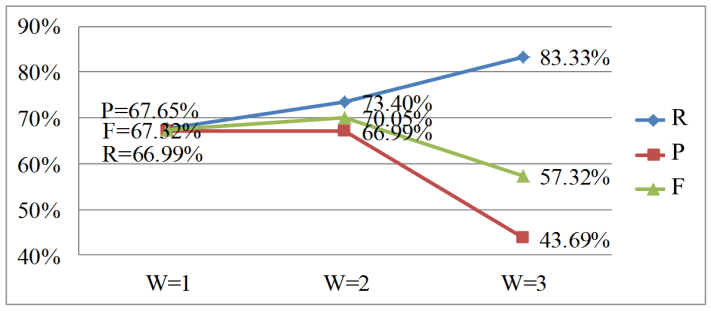
\includegraphics[height=150pt]{3-2.png}
\caption{Hotel语料评测结果}
\label{fig3-2}
\end{figure}

\begin{figure}[htp]
\centering
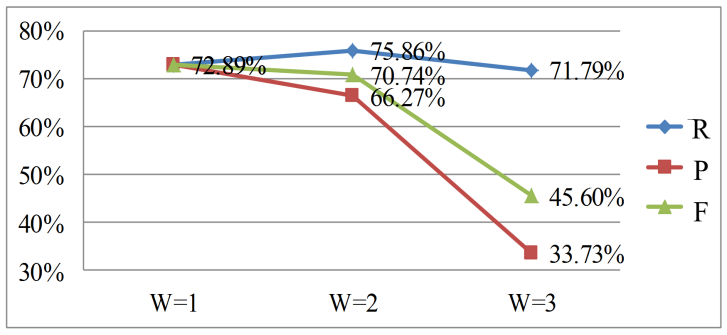
\includegraphics[height=150pt]{3-3.png}
\caption{Book语料评测结果}
\label{fig3-3}
\end{figure}

\begin{figure}[htp]
\centering
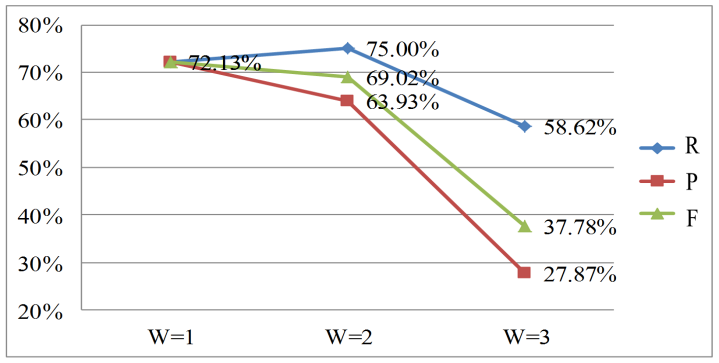
\includegraphics[height=170pt]{3-4.png}
\caption{NoteBook语料评测结果}
\label{fig3-4}
\end{figure}

\section{基于混合特征的情感词典扩展}
对基于语言特征的情感词典扩展方法和基于统计特征的情感词典扩展方法的实验结果进行仔细分析发现,采用语言特征无法进行情感极性计算的词语,可以采用统计特征进行处理;同样的,采用统计特征无法进行情感极性计算的词语,可以采用语言特征进行处理;两种方法可以相互补充。因此本文提出基于混合特征方法。

\subsection{基于混合特征的情感词极性计算}
基于混合特征的情感词语极性计算如算法~\ref{alg3-3}。将选取的情感词语集合分别采用两种方法进行极性计算,在将两种方法计算的极性值合成时,遵循以下原则:

\begin{enumerate}
\item 优先采用基于统计特征的方法计算出的情感极性值作为待标注词语的情感极性值。
\item 当采用基于统计特征的方法进行计算时,优先设置窗口大小为2,其次为1。
\item 当采用基于统计特征的方法无法对待评价词语进行情感计算时,采用基于语言特征的方法进行计算。
\end{enumerate}

\begin{algorithm}[htp]
\caption{基于混合特征的极性计算}
\label{alg3-3}
\begin{algorithmic}[1]
\REQUIRE ~~\\
待标注词语集,$\{w_1\}$;\\
极性已知词语集合,$\{w_2\}$;\\
连词集合,$\{c\}$;\\
每个词特征向量集合,$\{V(w)|w \in \{w_1\}\cup \{w_2\} \}$;

\FOR{每一待标注词语 $w_1 \in \{w_1\}$}
\STATE 依据算法~\ref{alg3-2}计算情感极性值
\IF{$
\begin{cases}
PosScore(w_1)=0\\
NegScore(w_1)=0
\end{cases}$}
\STATE 依据算法~\ref{alg3-1}计算情感极性值
\ENDIF
\STATE 根据情感值 $PosScore(w_1)$ 与$ NegScore(w_1) $判断极性;
\STATE 将$ w_1 $加入到集合$ \{w_2\} $;
\ENDFOR
\end{algorithmic}
\end{algorithm}

\subsection{实验}
对三个领域(Hotel、Book、NoteBook)的情感词典扩展实验结果如表~\ref{tab3-3}所示。

\begin{table}[htp]
\centering
\caption{各个领域性能评测结果}
\label{tab3-3}
\begin{tabular}{|l|l|l|l|}
\hline
 &正确率(P)& 召回率(R)& F值 \\
 \hline
 Hotel语料& 75.49\%& 74.76\%& 75.12\% \\
Book语料& 77.11\%& 77.11\%& 77.11\% \\
NoteBook语料&78.69\%& 78.69\%& 78.69\% \\
\hline
\end{tabular}
\end{table}
基于语言特征的情感词典扩展、基于统计特征的情感词典扩展和基于混合特征的情感词典扩展的实验评测结果对比情况如图~\ref{fig3-5}、图6~\ref{fig3-6}和图~\ref{fig3-7}所示,通过分析发现,基于混合特征的情感词典扩展方法的评测性能是在各个领域语料中均是最优的。

\begin{figure}[htp]
\centering
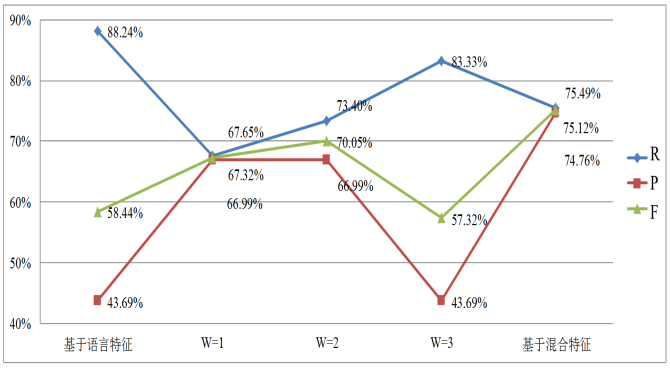
\includegraphics[height=190pt]{3-5.png}
\caption{Hotel语料评测结果综合比较}
\label{fig3-5}
\end{figure}

\begin{figure}[htp]
\centering
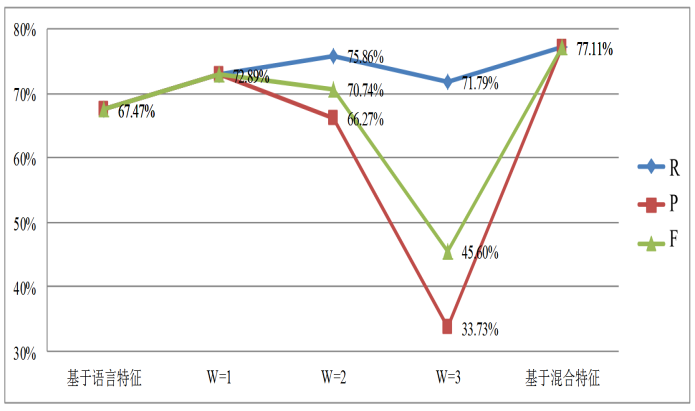
\includegraphics[height=190pt]{3-6.png}
\caption{Book语料评测结果综合比较}
\label{fig3-6}
\end{figure}

\begin{figure}[htp]
\centering
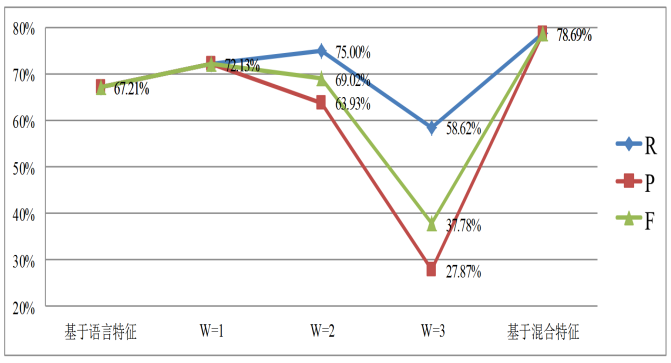
\includegraphics[height=190pt]{3-7.png}
\caption{NoteBook语料评测结果综合比较}
\label{fig3-7}
\end{figure}

\section{小结}
本章详细讨论了基于语料资源的中文情感词典扩展问题描述和方法设计,对基于语言特征的情感词典扩展和基于统计特征的情感词典扩展的关键技术分别进行了研究和算法实现,并提出了了基于混合特征的无监督的情感词典扩展方法。通过分析每个方法的实验结果,发现基于混合特征方法能够达到最好性能。
